\documentclass{article}
\usepackage{graphicx} % Required for inserting images
\usepackage{float}  % For wrapping text around figures
\usepackage{pgfplots}
\usepackage{amsmath} % Required for cases environment
\usepackage{mathrsfs}
\usepackage{amssymb} % For \mathbb
\usepackage{listings}
\usepackage{xcolor}

% Bibliography: classic BibTeX with the IEEEtran style (see Sources.bib and
% \bibliography near the end of the document).

\pgfplotsset{compat=1.18} % Ensure latest features

\graphicspath{ {./Figures/} }

\usepackage[a4paper, margin=1in]{geometry}
% Define style
\lstset{
    basicstyle=\ttfamily\small,
    keywordstyle=\color{blue},
    stringstyle=\color{red},
    commentstyle=\color{green!50!black},
    showstringspaces=false,
    breaklines=true
}

\title{130\,nm RGC-CD TIA Design Doc}
\author{Mathew Hanson}
\date{August 2026}

\begin{document}

\maketitle

\section{Introduction}
This report summarises the design of a transimpedance amplifier (TIA) I developed
as a member of the University of Waterloo's ASIC student design team during my Summer 2025
co-op semester. The TIA is the current-to-voltage front-end of a larger analog
matrix-vector multiplier (MVM). In that system the multiplication is carried out
by weighted current mirrors, so every column of a matrix $\mathbf{A}_{n\times n}$
produces an output current that must be converted to a voltage before it can be
digitised by an analog-to-digital converter (ADC).

Because an $n\times n$ MVM requires $n$ such converters, silicon area is the
dominant constraint. Providing each column with its own compact converter avoids the
bottleneck of a single centralised TIA fronted by an $n$-input current multiplexer.
This motivated a regulated-cascode (RGC) input stage rather than an operational-amplifier
based TIA: the RGC presents a low input impedance for current sensing while using far
fewer devices (and hence less area) than an op-amp design. The RGC stage is followed by
a capacitive-degeneration (CD) stage that extends the closed bandwidth. The overall
topology is adapted from the low-power TIA of \cite{Low-Power_TIA}. The complete
schematic, with the RGC input stage and CD stage highlighted, is shown in
Figure~\ref{fig:TIA Schem Full}.

\begin{figure}[H]
\centering
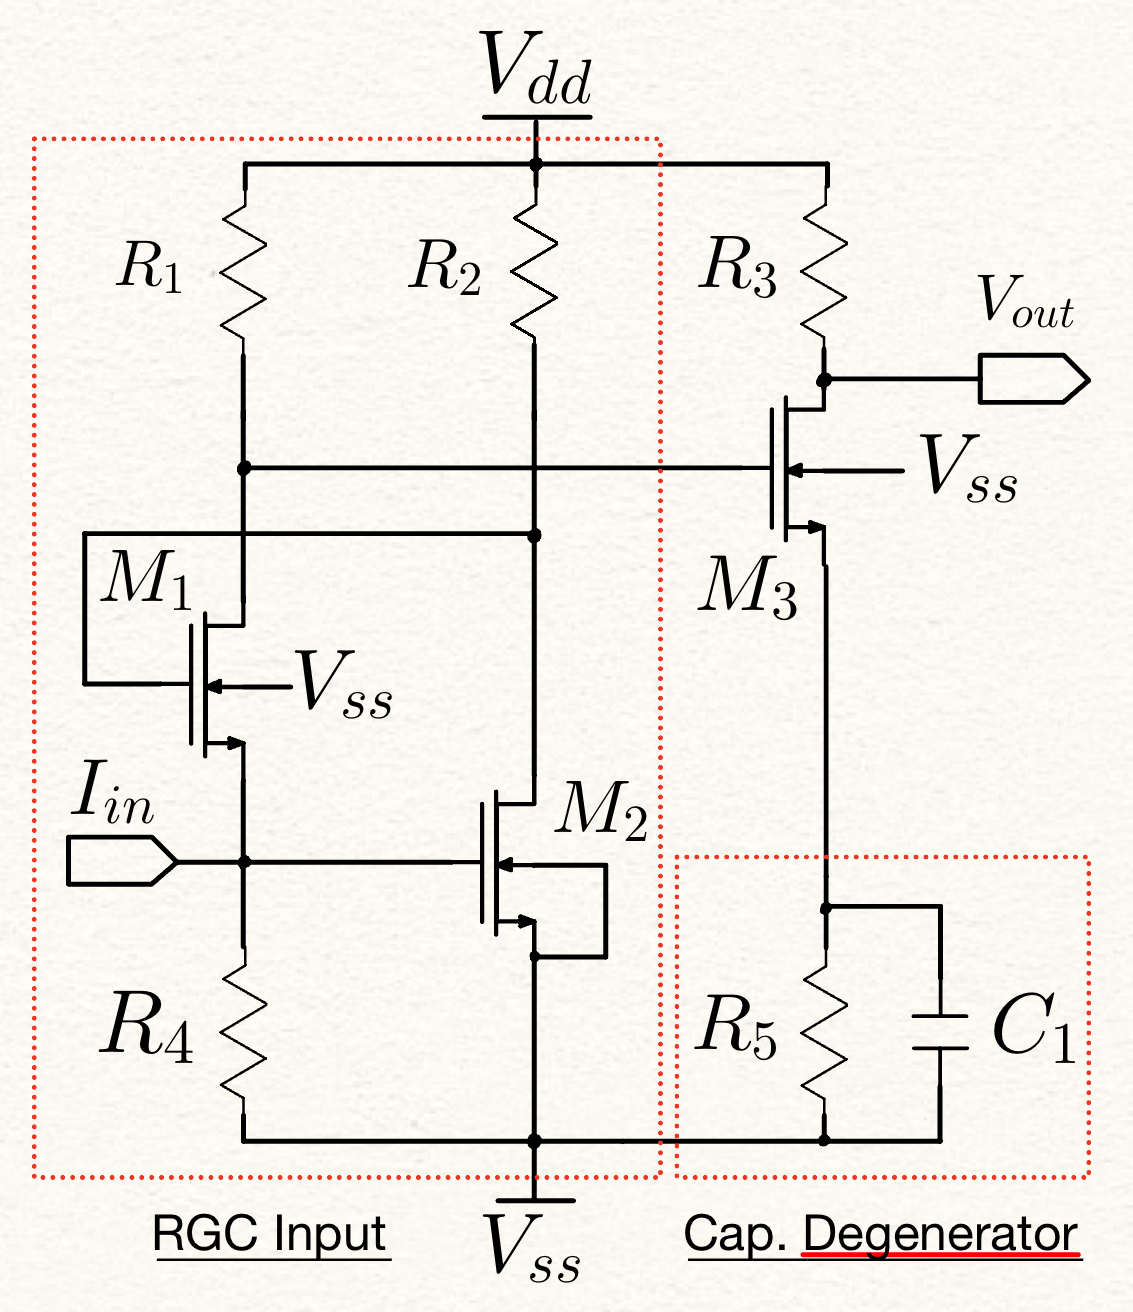
\includegraphics[width=8cm]{Figures/TIA_Schem_Full.png}
\caption{Complete RGC-CD TIA schematic (RGC input stage + capacitive-degeneration stage).}
\label{fig:TIA Schem Full}
\end{figure}

The entire design was carried out with an open-source flow: \texttt{xschem} for schematic
capture, \texttt{ngspice} for simulation, and \texttt{magic}/\texttt{klayout} for layout.
The topology of Figure~\ref{fig:TIA Schem Full} gives rise to the following net
identities, used without further comment throughout:
\begin{gather}
    V_{S_1}=V_{G_2}\\
    V_{G_1}=V_{D_2}\\
    V_{D_1}=V_{G_3}\\
    V_{out}=V_{D_3}
\end{gather}
As discussed in Section~\ref{sec:linearity}, the single-ended output biases this topology
asymmetrically and limits it to a largely unidirectional (single-sign) input current which works well with 
the current-mirror MVM front-end.

\section{Prior Work: The Original Baseline}
\label{sec:prior}
The circuit of Figure~\ref{fig:TIA Schem Full} was first designed and simulated against the
SKY130B $0.13\,\mu$m CMOS process to comply with the open-source TinyTapeout flow but never reached the layout stage. The
present document describes a subsequent revitalisation of that design on the SKY130A device
models. The topology is identical
between the two PDKs, only the sizing methodology and the device models differ. For
context, the headline results of the original SKY130B baseline are collected in
Table~\ref{tab:baseline}.

\begin{table}[H]
    \centering
    \caption{Original SKY130B baseline (identical topology, pre-layout, TT, $27^\circ$C).}
    \label{tab:baseline}
    \begin{tabular}{l|c|c} \hline
        \textbf{Parameter} & \textbf{Value} & \textbf{Units} \\ \hline
        Passive values ($R_1,R_2,R_4$)        & $2$              & $k\Omega$ \\ \hline
        Passive values ($R_3,R_5$)            & $6,\ 5.895$      & $k\Omega$ \\ \hline
        Degeneration cap $C_1$                & $450$            & $fF$ \\ \hline
        Full-TIA DC gain                      & $58.9\ (-884)$   & $dB\Omega\ (\Omega)$ \\ \hline
        RGC-only gain                         & $61.7$           & $dB\Omega$ \\ \hline
        Peaking                               & $\sim0.75$       & $dB$ \\ \hline
        RGC-only cutoff $f_{-3dB}$            & $66$             & $MHz$ \\ \hline
        RGC+CD cutoff $f_{-3dB}$              & $143$            & $MHz$ \\ \hline
        Power                                 & $1.06$           & $mW$ \\ \hline
        Input signal range                    & $-5$ to $+20$    & $\mu A$ \\ \hline
    \end{tabular}
\end{table}

The original sizing followed an overdrive-voltage ($V_{ov}$) approach: every device
was sized from the square-law relation
$I_D=\tfrac{1}{2}k'\tfrac{W}{L}V_{ov}^2$ with a fixed $V_{ov}=0.2\,V$, an assumed
$V_{th}=0.4\,V$ (LVT), and an assumed process transconductance $k'=60\ \mu A/V^2$. This is
simple to hand-calculate, but it assumes strong-inversion square-law behaviour and a
transconductance parameter that is not, in practice, well known before characterisation. On
the faster SKY130A models the assumed $k'$ proved inaccurate (the measured RGC gain landed on
the hand-calculated $\sim66\,dB\Omega$ rather than the $61.7\,dB\Omega$ originally
simulated), and the frequency-dependent quantities did not port at all: the intrinsic RGC
pole moved from the anticipated $66\,MHz$ up to $\approx2\,GHz$.

For the revitalisation the design was therefore re-derived from the ground up using a
$g_m/I_D$ methodology, in which every device is sized from measured
current-density and speed data rather than from an assumed square-law constant. The full
$g_m/I_D$ design flow, small-signal analysis, and SKY130A simulation results are the subject
of Section~\ref{sec:flow}.

\section{RGC-CD Design Flow ($g_m/I_D$, SKY130A)}
\label{sec:flow}

\subsection{$g_m/I_D$ Design Methodology}
\label{sec:gmid}
The $g_m/I_D$ method sizes each transistor from measured device curves rather than from an
assumed square-law $k'$. A unit-width device is swept over $V_{GS}$ at a fixed
$|V_{DS}|=V_{DD}/2$, and per operating point the small-signal quantities $g_m$, $g_{ds}$,
$C_{gg}$ are extracted directly from the BSIM instance inside the SKY130 model. Because
$g_m/I_D$ and the current density $J_D=I_D/W$ are essentially width-independent, a single
unit device characterises the whole family.

The operating-point choice trades efficiency against speed. A high $g_m/I_D$
(weak/moderate inversion) maximises transconductance per unit current and intrinsic gain
$g_m r_o$ but gives a low transit frequency $f_T$. A low $g_m/I_D$ (strong inversion)
does the opposite. Figure~\ref{fig:gmid nfet} shows the four master charts for the LVT nfet
used throughout the RGC-CD signal path, and Figure~\ref{fig:gmid overlay} overlays the nfet
against the pfet at the channel lengths the candidate topologies actually use.

\begin{figure}[H]
\centering
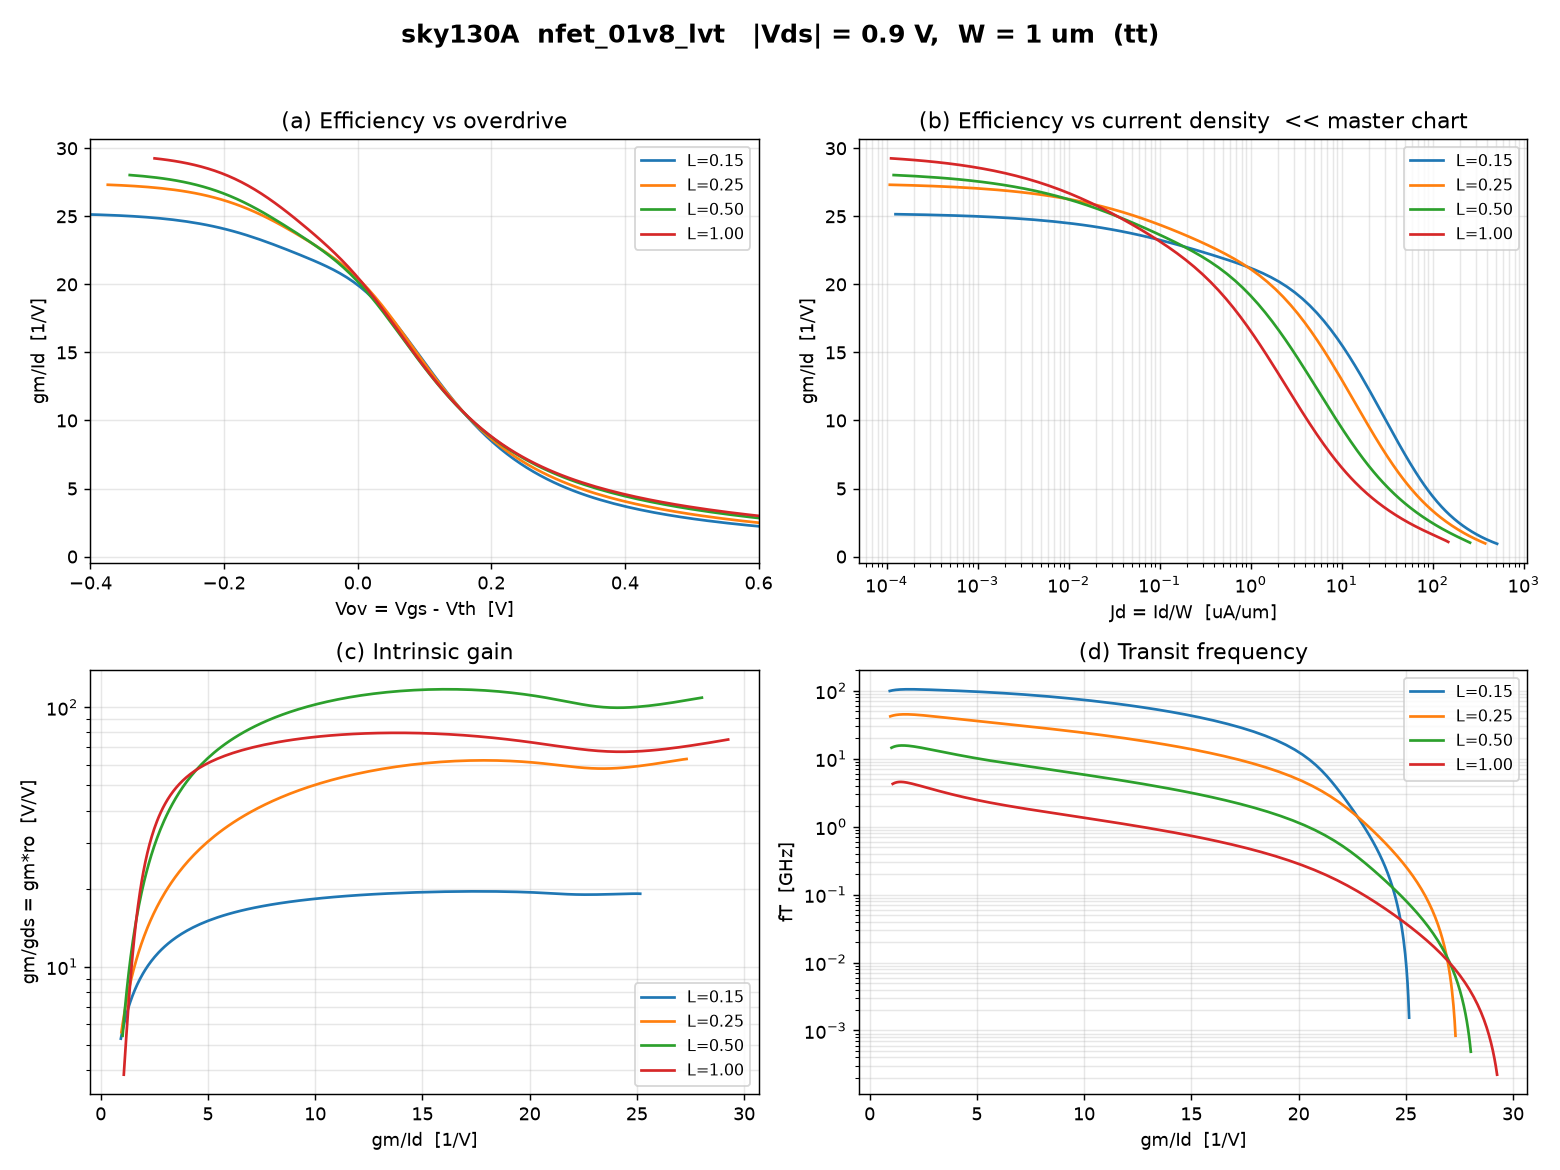
\includegraphics[width=13cm]{Figures/gmid_nfet_01v8_lvt.png}
\caption{$g_m/I_D$ master charts for the SKY130A LVT nfet ($|V_{DS}|=0.9\,V$): (a) efficiency
vs.\ overdrive, (b) efficiency vs.\ current density $J_D$ (the master sizing chart),
(c) intrinsic gain $g_m r_o$, and (d) transit frequency $f_T$, each vs.\ $g_m/I_D$.}
\label{fig:gmid nfet}
\end{figure}

\begin{figure}[H]
\centering
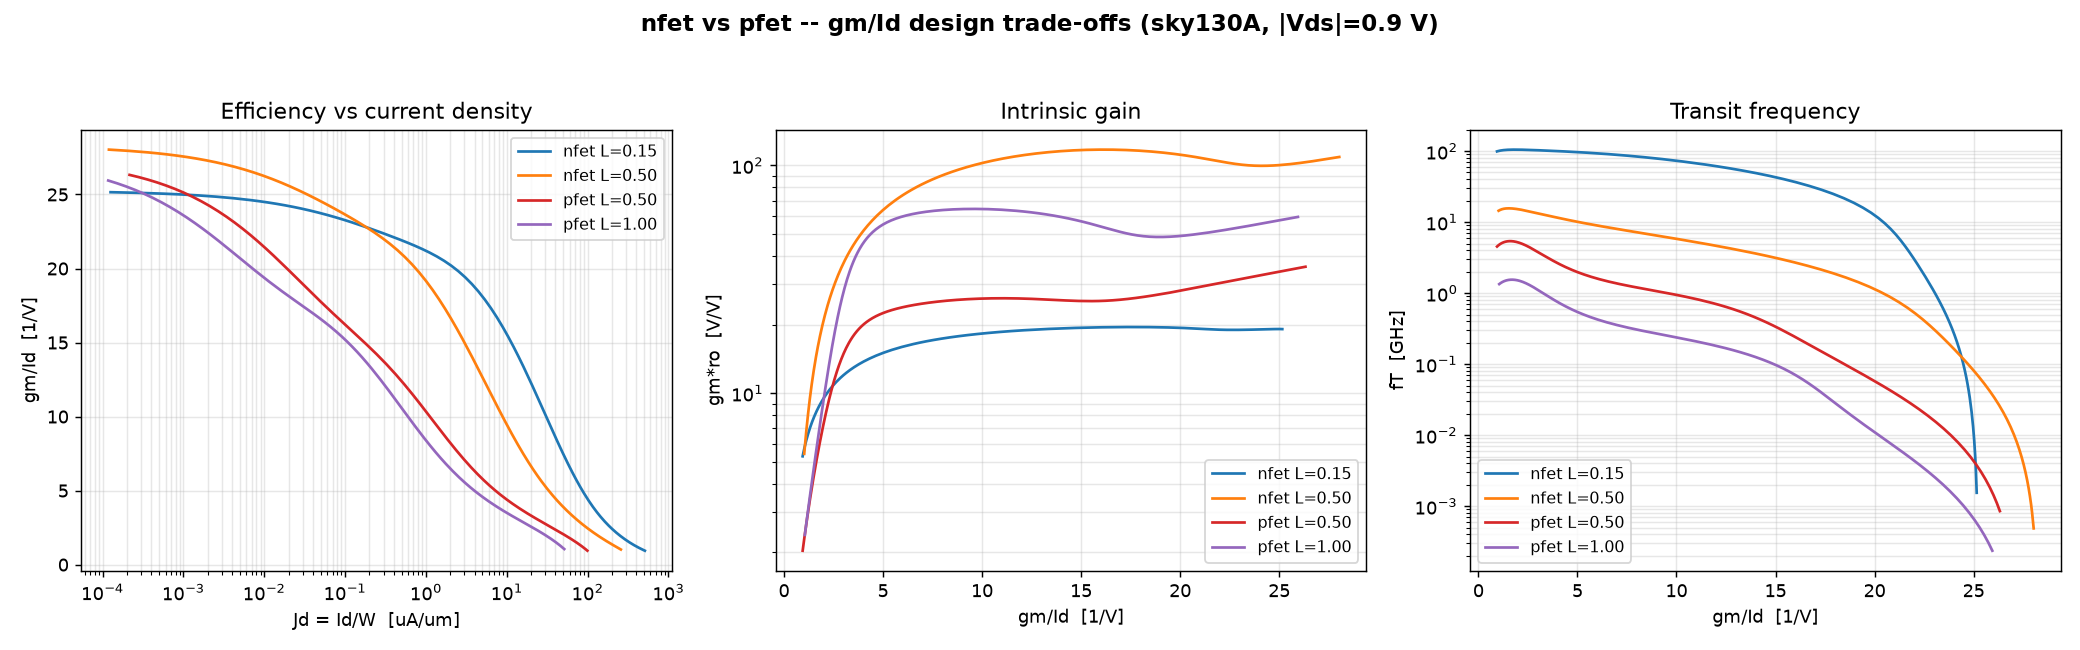
\includegraphics[width=13cm]{Figures/gmid_overlay_nfet_vs_pfet.png}
\caption{Cross-device $g_m/I_D$ trade-offs (efficiency, intrinsic gain, $f_T$) for the nfet
and pfet at the lengths the RGC-CD front-end uses.}
\label{fig:gmid overlay}
\end{figure}

The cascode/auxiliary devices $M_1,M_2$ were placed at $g_m/I_D=18\,V^{-1}$ (moderate
inversion, a balance of loop gain and speed), and the degeneration device $M_3$ at
$g_m/I_D=22\,V^{-1}$ (slightly more efficient, since its speed is set by the degeneration
network rather than by $f_T$). Reading $J_D$, $g_m r_o$, and $f_T$ off the charts at the
chosen bias currents yields the sizing summarised in Table~\ref{tab:gmid sizing}. All devices
use the minimum $L=0.15\,\mu$m. Each is to be laid out multi-finger for implementation, with
negligible electrical effect (Section~\ref{sec:fingering}).

\begin{table}[H]
    \centering
    \caption{$g_m/I_D$ device sizing (SKY130A LVT nfet, $L=0.15\,\mu$m).}
    \label{tab:gmid sizing}
    \begin{tabular}{c|c|c|c|c|c|c} \hline
        \textbf{Device} & \textbf{$I_D$ [$\mu$A]} & \textbf{$g_m/I_D$ [$V^{-1}$]} &
        \textbf{$W$ [$\mu$m]} & \textbf{$g_m$ [mS]} & \textbf{$g_m r_o$} & \textbf{$f_T$ [GHz]} \\ \hline
        $M_1$ (cascode)        & 60 & 18 & 7.3  & 1.08 & 14.4 & 36.0 \\ \hline
        $M_2$ (aux CS)         & 55 & 18 & 7.9  & 0.99 & 14.9 & 29.8 \\ \hline
        $M_3$ (degeneration)   & 40 & 22 & 19.1 & 0.88 & 14.3 & 12.2 \\ \hline
    \end{tabular}
\end{table}

The passive network that biases this sizing (and shapes the response of
Section~\ref{sec:tf}) is $R_1=6.5\,k\Omega$, $R_2=6\,k\Omega$, $R_3=4\,k\Omega$,
$R_4=9\,k\Omega$, $R_5=22.5\,k\Omega$, and $C_1=178\,fF$. The front-end is deliberately
current-starved: a large $R_5$ with a low $I_3$ maximises $g_{m3}R_5$, which (as shown below)
pushes the degeneration pole high, while $R_4=9\,k\Omega$ keeps the input node biased for
adequate saturation margin.

\subsection{Small-Signal Transfer Function and Pole/Zero Set}
\label{sec:tf}
\subsubsection{RGC front-end}
The auxiliary common-source amplifier $M_2$ ($V_{G_2}=V_{S_1}$, load $R_2$) provides a
regulating gain
\begin{gather}
    A_{aux}=g_{m2}R_2\approx 5.9\ V/V.
\end{gather}
This gain boosts the shunt feedback around $M_1$, lowering the input impedance seen by the
injected signal current to
\begin{gather}
    Z_{in}=\frac{1}{g_{m1}(1+A_{aux})}\ \Big\|\ R_4 \approx 132\ \Omega.
\end{gather}
The signal current flows through $M_1$ into $R_1$, so the front-end transimpedance to the RGC
output node $V_{D_1}$ is set (to first order) by the load resistor, $Z_{T,\text{RGC}}\approx R_1$.

\subsubsection{Capacitive-degeneration stage}
The CD stage is a common-source amplifier $M_3$ whose source is degenerated by the parallel
network $Z_5(s)=R_5\|(1/sC_1)=R_5/(1+sR_5C_1)$. Writing KCL at $V_{out}$ and $V_{S_3}$
(small-signal model in Figure~\ref{fig:Small Signal M3}),
\begin{gather}
    \frac{V_{out}-V_{S_3}}{r_{o3}}+\frac{V_{out}}{R_3}+g_{m3}(V_{G_3}-V_{S_3})=0
        \label{eq:nodal at v_out}\\
    -g_{m3}(V_{G_3}-V_{S_3})+\frac{V_{S_3}-V_{out}}{r_{o3}}+\frac{V_{S_3}}{Z_5(s)}=0
        \label{eq:nodal at v_s3}
\end{gather}
\begin{figure}[H]
\centering
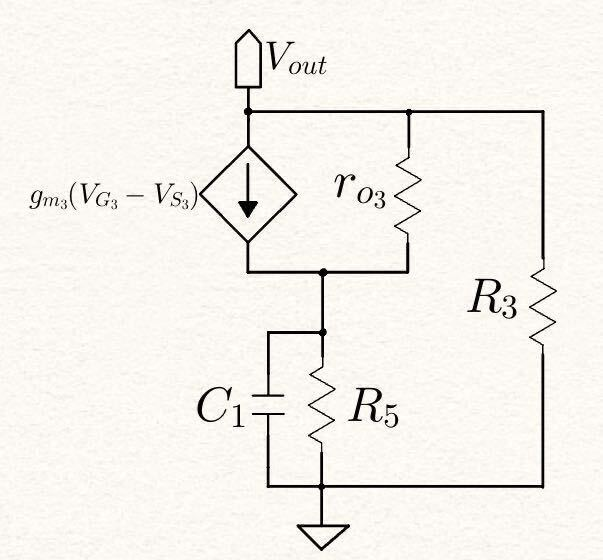
\includegraphics[width=8cm]{Figures/TIA_Schem_M3.png}
\caption{Small-signal model of the capacitive-degeneration stage ($M_3$ degenerated by $R_5\|C_1$).}
\label{fig:Small Signal M3}
\end{figure}
Eliminating $V_{S_3}$ gives a single-zero, single-pole response
\begin{gather}
    A_{CD}(s)=A_0\,\frac{1+s/\omega_z}{1+s/\omega_p},\qquad
    A_0=\frac{g_{m3}R_3}{1+g_{m3}R_5},\\
    \omega_z=\frac{1}{R_5C_1},\qquad
    \omega_p=\frac{1+g_{m3}R_5}{R_5C_1}\approx\frac{g_{m3}}{C_1}.
\end{gather}
Because $g_{m3}R_5\gg1$, the pole sits well above the zero: the stage produces a rising (peaking)
response between $\omega_z$ and $\omega_p$ that is used to extend the closed bandwidth. The CD
stage is a common-source amplifier, so $A_0$ is in fact negative: it both attenuates
($|A_0|\approx0.17$, the source degeneration $g_{m3}R_5$ dividing the gain down) and inverts the
overall TIA output. The load-resistor front-end contributes the transimpedance magnitude, the
common-source stage its sign. The positive $A_0$ written above is thus a magnitude, as is the
$Z_{T,DC}$ term below.

\subsubsection{Loaded transfer function}
In the deployed system the input node carries the MVM current-mirror capacitance
($C_T\approx500\,fF$) and the output drives an ADC sampling input ($C_L\approx1\,pF$). These
introduce two additional load-induced poles, one at the input node and one at the output
node:
\begin{gather}
    \omega_{in}=\frac{1}{Z_{in}C_T},\qquad
    \omega_{out}=\frac{1}{R_3C_L}.
\end{gather}
Collecting the front-end, CD stage, internal nodes and loads, the full first-order
transimpedance is
\begin{gather}
    Z_T(s)=\underbrace{R_1\,\frac{g_{m3}R_3}{1+g_{m3}R_5}}_{\textstyle Z_{T,DC}}
    \cdot
    \frac{1+s/\omega_z}
         {\left(1+\dfrac{s}{\omega_{in}}\right)
          \left(1+\dfrac{s}{\omega_{aux}}\right)
          \left(1+\dfrac{s}{\omega_{D1}}\right)
          \left(1+\dfrac{s}{\omega_{p}}\right)
          \left(1+\dfrac{s}{\omega_{out}}\right)}.
\end{gather}
Evaluating each singularity at the sizing of Table~\ref{tab:gmid sizing} gives the pole/zero set
of Table~\ref{tab:polezero}. The internal-node poles $\omega_{D1}$ (transimpedance node) and
$\omega_{aux}$ (aux-loop node) are gate-capacitance-dominated estimates.

\begin{table}[H]
    \centering
    \caption{First-order pole/zero set of the loaded transimpedance ($g_m/I_D$ design,
    $C_T=500\,fF$, $C_L=1\,pF$).}
    \label{tab:polezero}
    \begin{tabular}{l|c|c|l} \hline
        \textbf{Singularity} & \textbf{Type} & \textbf{Frequency} & \textbf{Expression} \\ \hline
        $f_z$   (CD zero)          & zero & $40\ MHz$   & $1/(2\pi R_5 C_1)$ \\ \hline
        $f_{out}$ (output/load)    & pole & $40\ MHz$   & $1/(2\pi R_3 C_L)$ \\ \hline
        $f_p$   (CD pole)          & pole & $827\ MHz$  & $(1+g_{m3}R_5)/(2\pi R_5 C_1)$ \\ \hline
        $f_{D1}$ (transimp.\ node) & pole & $2.13\ GHz$ & $1/(2\pi R_1 C_{D1})$ \\ \hline
        $f_{in}$ (input/load)      & pole & $2.42\ GHz$ & $1/(2\pi Z_{in} C_T)$ \\ \hline
        $f_{aux}$ (aux loop)       & pole & $5.56\ GHz$ & $1/(2\pi R_2 C_{D2})$ \\ \hline
    \end{tabular}
\end{table}

\subsection{$s$-Plane View: Zero--Pole Cancellation}
\label{sec:splane}
Every singularity in Table~\ref{tab:polezero} is real and lies in the left-half plane, so the
$s$-plane collapses onto the negative real axis (Figure~\ref{fig:splane}). The value of the CD
stage is now explicit. Without any degeneration capacitor the response would roll off at the
lowest pole, which is the output/load pole $f_{out}=1/(2\pi R_3 C_L)\approx40\,MHz$ set by the
$1\,pF$ ADC load. The degeneration capacitor is sized so that the CD zero lands on that
load pole,
\begin{gather}
    R_5 C_1 = R_3 C_L\quad\Longrightarrow\quad f_z=f_{out}=40\ MHz,
\end{gather}
which cancels it. With the load pole removed, the dominant pole role passes to the CD pole
$f_p\approx827\,MHz$ and the $\sim2\,GHz$ intrinsic cluster ($f_{D1}, f_{in}$), so the closed
bandwidth is extended by more than a decade. The input-load pole $f_{in}$ and the aux-loop
pole $f_{aux}$ sit even higher and do not limit the response.

\begin{figure}[H]
\centering
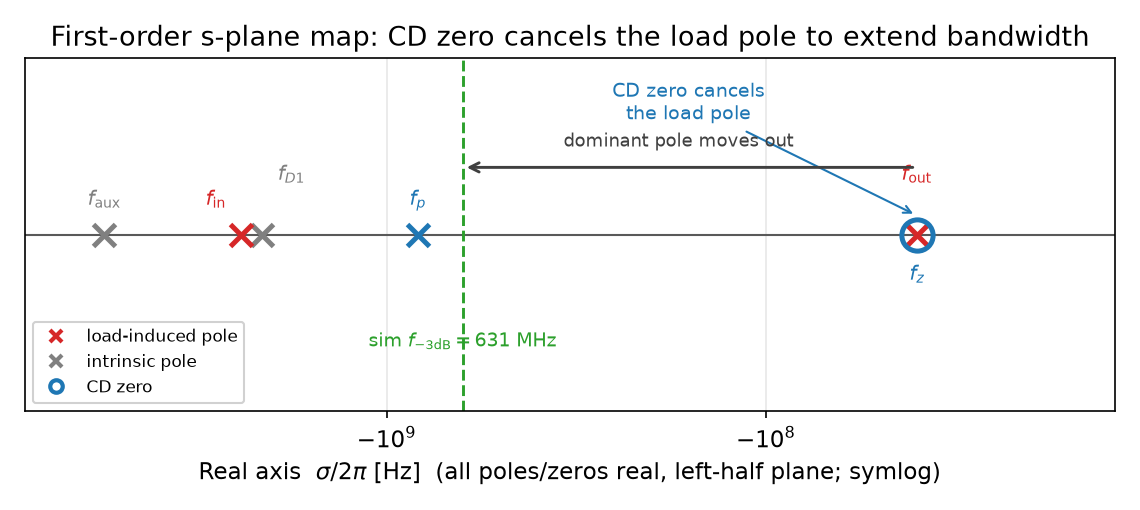
\includegraphics[width=14cm]{Figures/tia_splane.png}
\caption{First-order $s$-plane map of the loaded transimpedance. The CD zero $f_z$ is placed on
the output (load) pole $f_{out}$. Cancelling it moves the dominant pole out to the $\sim$GHz
cluster, extending the bandwidth to the simulated $631\,MHz$.}
\label{fig:splane}
\end{figure}

\subsection{Simulated DC and Frequency Response}
\label{sec:acresults}
The $g_m/I_D$ sizing was verified in ngspice on the SKY130A models. Every device settles in
saturation. The operating-point currents drift modestly from the sizing targets
($I_1,I_2,I_3\approx68/80/33\,\mu A$ vs.\ $60/55/40\,\mu A$ targeted), giving a total supply
current of $0.18\,mA$ and a power of
\begin{gather}
    P_{TIA}=V_{DD}\cdot I_{tot}=(1.8\,V)(0.18\,mA)\approx0.33\ mW,
\end{gather}
a $3\times$ reduction from the original $1.06\,mW$ baseline. The simulated DC transimpedance is
$59.4\,dB\Omega$ ($933\,\Omega$), with the output parked high at a nominal $V_{out}\approx1.67\,V$
(see Section~\ref{sec:linearity}).

Figure~\ref{fig:freq response} isolates the capacitive degenerator by comparing the loaded
response with and without $C_1$. With only resistive degeneration ($C_1=0$) the transimpedance
rolls off at the bare output/load pole at $\approx39\,MHz$. Restoring $C_1$ cancels that pole
and extends the $-3\,dB$ bandwidth to $631\,MHz$, a $\sim16\times$ extension at unchanged DC
gain and with negligible ($<0.1\,dB$) peaking. This is exactly the zero--pole cancellation of
Section~\ref{sec:splane}. The remaining two overlays in the figure, the folded real-device
netlist and the parasitic-extracted layout, preview the physical implementation of
Section~\ref{sec:physical}. Both preserve this flat frequency response with only a modest bandwidth trim.

\begin{figure}[H]
\centering
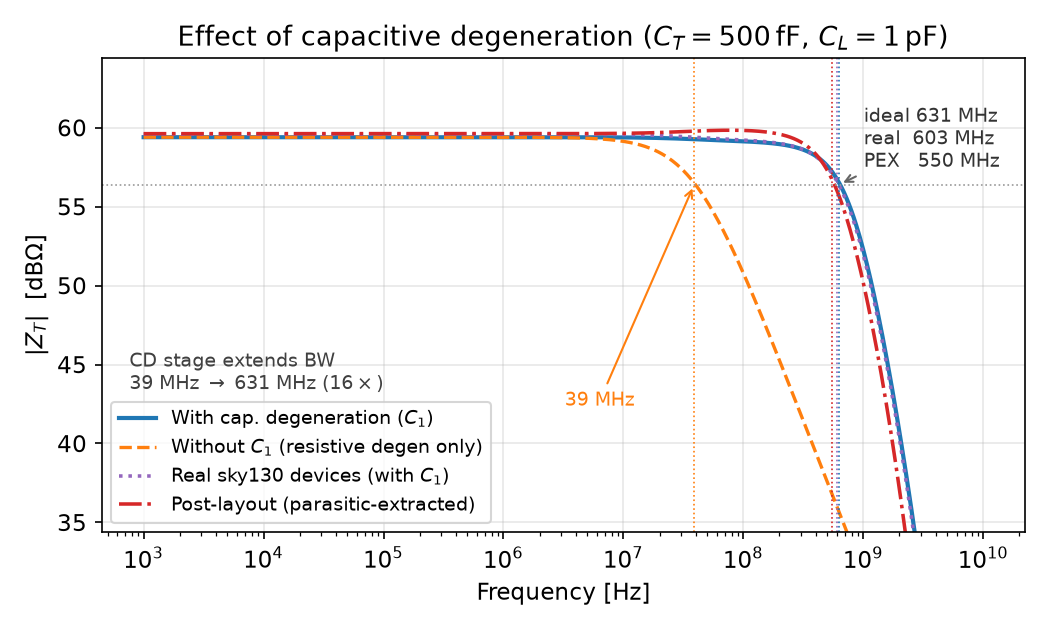
\includegraphics[width=13cm]{Figures/tia_freq_response_loaded.png}
\caption{Effect of the capacitive-degeneration stage on the loaded transimpedance
(SKY130A, TT, $27^\circ$C, $C_T=500\,fF$ input, $C_L=1\,pF$ ADC load). The ideal
single-finger design is shown with and without $C_1$. Overlaid are the folded
real-device and post-layout parasitic-extracted responses of
Section~\ref{sec:physical}, which retain the flat DC gain while trimming the
$-3\,dB$ bandwidth from $631$ to $603$ and $556\,MHz$ respectively.}
\label{fig:freq response}
\end{figure}

It is worth stressing that this compensation is load- and process-dependent: the CD zero must
be placed on whichever pole actually dominates (here the ADC-load pole), and re-centred if the
target load or bias changes. This is precisely why the original $C_1=450\,fF$ (sized on SKY130B
for a $66\,MHz$ pole) over-peaks on the faster SKY130A devices, and why $C_1$ is exposed as a
tunable parameter in the reconstructed netlist. In an unloaded testbench, with the RGC
pole near $2\,GHz$ and no load pole for the zero to cancel, the same $C_1$ produces a large
($\sim{+}17\,dB$) resonant peak.

\subsection{Loop Stability}
\label{sec:stability}
Because the RGC relies on the local $M_1$--$M_2$ regulation loop, its stability must be checked
at the deployed operating point. Figure~\ref{fig:phase margin} shows the loop gain and phase
under the same $C_T/C_L$ loading. The loop has a DC gain of $\approx12\,dB$ and crosses unity
gain near $940\,MHz$ with $\approx130^\circ$ of phase margin, so the flat extended response of
Section~\ref{sec:acresults} is a well-damped operating point rather than a lightly-damped
resonance.

\begin{figure}[H]
\centering
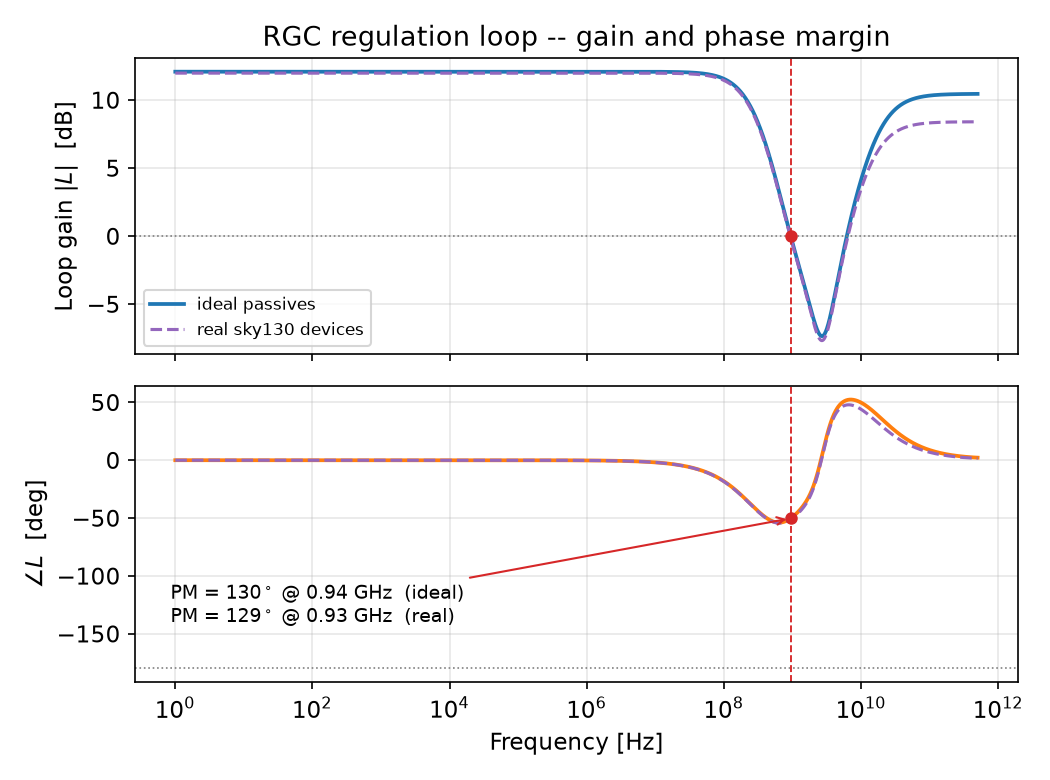
\includegraphics[width=13cm]{Figures/tia_phase_margin.png}
\caption{RGC regulation-loop gain and phase margin (SKY130A, TT, $27^\circ$C, with $C_T=500\,fF$
input and $C_L=1\,pF$ load).}
\label{fig:phase margin}
\end{figure}

\subsection{Input Linearity and the Negative-Current Limitation}
\label{sec:linearity}
The input current is injected at the source of $M_1$, a low-impedance node ($Z_{in}\approx132\,\Omega$)
held near $0.6\,V$ by the auxiliary loop, while the single-ended output is biased above
mid-rail ($\sim1.67\,V$). The available output swing is therefore asymmetric: a positive
(sourcing) input pulls $V_{out}$ down toward $V_{SS}$ (ample headroom), whereas a negative input
pushes $V_{out}$ up toward $V_{DD}$ (limited headroom). At the system level a current-mirror MVM
front-end can only source current in one direction, so realising genuinely bidirectional (signed)
input currents would require additional current-steering circuitry.

The core amplifier is more robust than the original $-5/+20\,\mu A$ signal
window suggests. The DC linearity sweep of Figure~\ref{fig:linearity} shows the small-signal
transimpedance staying within $10\%$ of its nominal value over roughly $-85$ to $+65\,\mu A$,
with hard clipping only beyond those points (as $V_{out}\!\rightarrow\!V_{DD}$ for large negative
input, and $V_{out}\!\rightarrow\!V_{SS}$ for large positive input). The original $-5/+20\,\mu A$
figures thus represent the signal window chosen to match the expected (largely unidirectional)
MVM currents rather than a hard electrical limit of the core.

\begin{figure}[H]
\centering
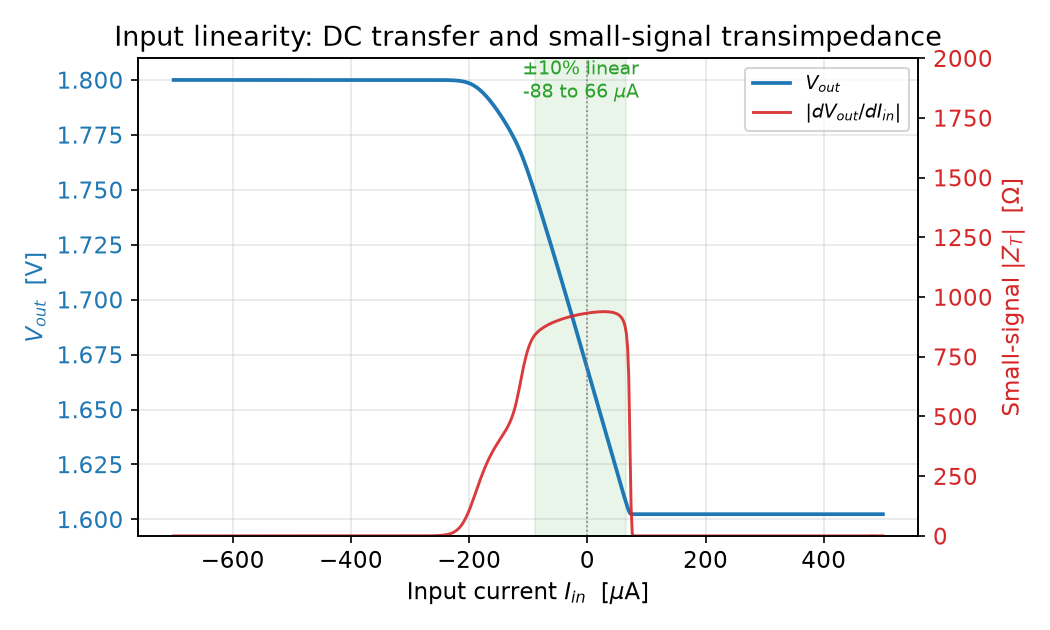
\includegraphics[width=13cm]{Figures/tia_linearity.png}
\caption{Input linearity: DC transfer $V_{out}(I_{in})$ and small-signal transimpedance vs.\
operating point (SKY130A, TT, $27^\circ$C).}
\label{fig:linearity}
\end{figure}

\subsection{Input-Referred Noise}
\label{sec:noise}
The input-referred current noise is obtained by integrating the input-referred noise spectral
density over the design band. Integrating over the loaded band ($1\,kHz$ to the
$631\,MHz$ $-3\,dB$ point of Section~\ref{sec:acresults}) gives
\begin{gather}
    \bar{I}_{n,rms}\big|_{T=27^\circ C}
    =\sqrt{\int_{1\,kHz}^{631\,MHz}\!\overline{i_n^2}(f)\,df}
    \approx158\ nA_{rms}.
\end{gather}
This is substantially larger than the $\sim73\,nA_{rms}$ obtained over the old $\sim140\,MHz$
band, for two compounding reasons: the band is more than $4\times$ wider, and the input-referred
density rises at high frequency as the transimpedance $|Z_T|$ rolls off (input-referred
noise $=$ output noise $/\,|Z_T|$). The spectral density is shown in
Figure~\ref{fig:noise spectrum}: a $1/f$ (flicker) roll-off below ${\sim}20\,kHz$ down to a white
thermal floor of ${\approx}9.6\ pA/\sqrt{Hz}$, then the high-frequency rise from the
transimpedance roll-off. The temperature dependence is given in Table~\ref{tab:noise vs temp}.
Unlike the baseline design, integrating to a fixed $631\,MHz$ makes the total noise
increase with temperature, as expected for a thermally-dominated floor.

\begin{figure}[H]
\centering
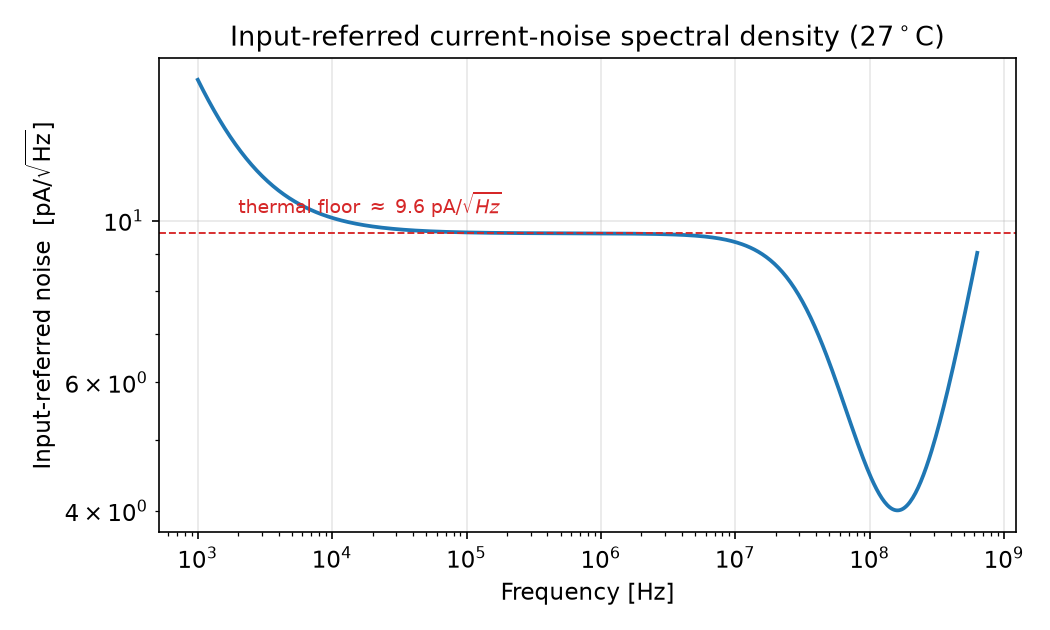
\includegraphics[width=12cm]{Figures/tia_noise_spectrum.png}
\caption{Input-referred current-noise spectral density (SKY130A, TT, $27^\circ$C, loaded).}
\label{fig:noise spectrum}
\end{figure}

\begin{table}[H]
    \centering
    \caption{Input-referred noise vs.\ temperature (integrated $1\,kHz$--$631\,MHz$, loaded).}
    \label{tab:noise vs temp}
    \begin{tabular}{c|c|c} \hline
        \textbf{Temp [$^\circ$C]} & \textbf{$\bar{I}_{n,rms}$ [$nA_{rms}$]} & \textbf{$V_{o,n}$ [$\mu V_{rms}$]} \\ \hline
        27 & 158.2 & 127.8 \\ \hline
        45 & 165.3 & 131.7 \\ \hline
        75 & 177.1 & 137.8 \\ \hline
    \end{tabular}
\end{table}

\subsection{Device Fingering for Layout}
\label{sec:fingering}
For physical implementation the signal devices will be drawn multi-finger: $M_1$, $M_2$, and the
wide degeneration device $M_3$ each with $n_f=4$ fingers (per-finger widths of
$1.8$, $2.0$ and $4.8\,\mu$m). The electrical design of record above is characterised at
$n_f=1$. Folding is a layout choice, not an electrical one: the total gate width, and hence
$g_m$, $I_D$, and every gain and pole of Table~\ref{tab:gmid sizing}, is unchanged. The motivation is purely physical: a single-finger $M_3$ is a
$19.1\,\mu$m$\,\times\,0.15\,\mu$m sliver ($127{:}1$ aspect ratio) that is awkward to place and
route, whereas four $4.8\,\mu$m fingers form a compact cell whose adjacent fingers
share source/drain diffusions. Folding also enables interdigitated / common-centroid placement
of the matched $M_1$--$M_2$ regulation pair.

Re-simulating the folded netlist confirms the change is electrically negligible
(Table~\ref{tab:fingering}). The redistributed source/drain junction geometry nets a small
increase in internal-node parasitic capacitance, which lowers the loaded bandwidth by $\sim4\%$
($631\rightarrow603\,MHz$) and, at a \emph{common} integration band, raises the input-referred
noise by $\sim2.5\%$. DC gain, phase margin and power are unchanged to rounding. Integrated to
the folded variant's own $603\,MHz$ $-3\,dB$ point, its input-referred noise would be
$154.5\,nA_{rms}$.

Two caveats frame this result. First, the pre-layout SKY130 device models do \emph{not} include
distributed gate resistance ($r_{gate}$ is disabled), so the principal benefit of fingering
(the $\propto 1/n_f^2$ collapse of gate-resistance thermal noise, which for a single-finger $M_3$
would otherwise rival its channel noise) does not appear in these numbers. The cap-only
parasitic extraction of Section~\ref{sec:pex} likewise omits it, so capturing that benefit will
require a full RC extraction. Second, the small bandwidth/noise
penalty seen here sits well within the SKY130A-vs-B model spread already noted in
Section~\ref{sec:prior}. Fingering is therefore adopted as electrically free pre-layout and
net-beneficial after extraction.

\begin{table}[H]
    \centering
    \caption{Effect of device fingering on the loaded design (SKY130A, TT, $27^\circ$C).}
    \label{tab:fingering}
    \begin{tabular}{l|c|c} \hline
        \textbf{Metric} & \textbf{Single-finger ($n_f{=}1$)} & \textbf{Folded ($n_f{=}4$)} \\ \hline
        DC transimpedance [$dB\Omega$]      & 59.4  & 59.6  \\ \hline
        Loaded $f_{-3dB}$                   & $631\,MHz$ & $603\,MHz$ \\ \hline
        Peaking [dB]                        & $<0.1$ & $<0.1$ \\ \hline
        Loop phase margin                   & $130^\circ$ & $129^\circ$ \\ \hline
        Input-referred noise$^\dagger$ [$nA_{rms}$] & 158.2 & 162.1 \\ \hline
        Power [mW]                          & 0.33  & 0.33  \\ \hline
    \end{tabular}
    \\[2pt]
    {\footnotesize $^\dagger$ integrated over a \emph{common} $1\,kHz$--$631\,MHz$ band to isolate
    the device effect. Over each design's own $-3\,dB$ band the folded figure is $154.5\,nA_{rms}$.}
\end{table}

\section{Physical Implementation}
\label{sec:physical}
With the pre-layout design frozen, the TIA was carried through schematic capture, physical
layout, layout-versus-schematic (LVS) verification, and parasitic extraction (PEX) on the
open-source SKY130A flow inside the IIC-OSIC-TOOLS container. This section documents that
back-end flow and quantifies the loaded gain and bandwidth once real devices and layout
parasitics are accounted for.

\subsection{Schematic Capture (\texttt{xschem})}
\label{sec:xschem}
The design of record was entered in \texttt{xschem} to serve as the single source for both
pre-layout simulation and the LVS reference. Figure~\ref{fig:xschem} shows the captured
schematic. The three signal devices $M_1$--$M_3$ are \texttt{nfet\_01v8\_lvt} instances drawn
multi-finger ($n_f=4/4/4$) at the widths of Table~\ref{tab:gmid sizing}. The bias network uses
\texttt{res\_high\_po\_0p35} for $R_1$--$R_4$ and the higher-sheet \texttt{res\_xhigh\_po\_0p69}
for the large $R_5$ (design target $22.5\,k\Omega$, $\approx22.8\,k\Omega$ as drawn). The degeneration capacitor $C_1$ is a
\texttt{cap\_mim\_m3\_1} MIM ($17\times5\,\mu$m, $178\,fF$). Net labels follow the identities of
the Introduction ($d_1=V_{G_3}$, $d_2=V_{G_1}$, $s_3=V_{S_3}$), and the ports are \texttt{Iin},
\texttt{Vout}, \texttt{VDD}, \texttt{VSS}. Two dummy resistors (\texttt{Rdum1}, \texttt{Rdum2},
tied to \texttt{VSS}) flank the active bank so the matched resistors see identical neighbours.

\begin{figure}[H]
\centering
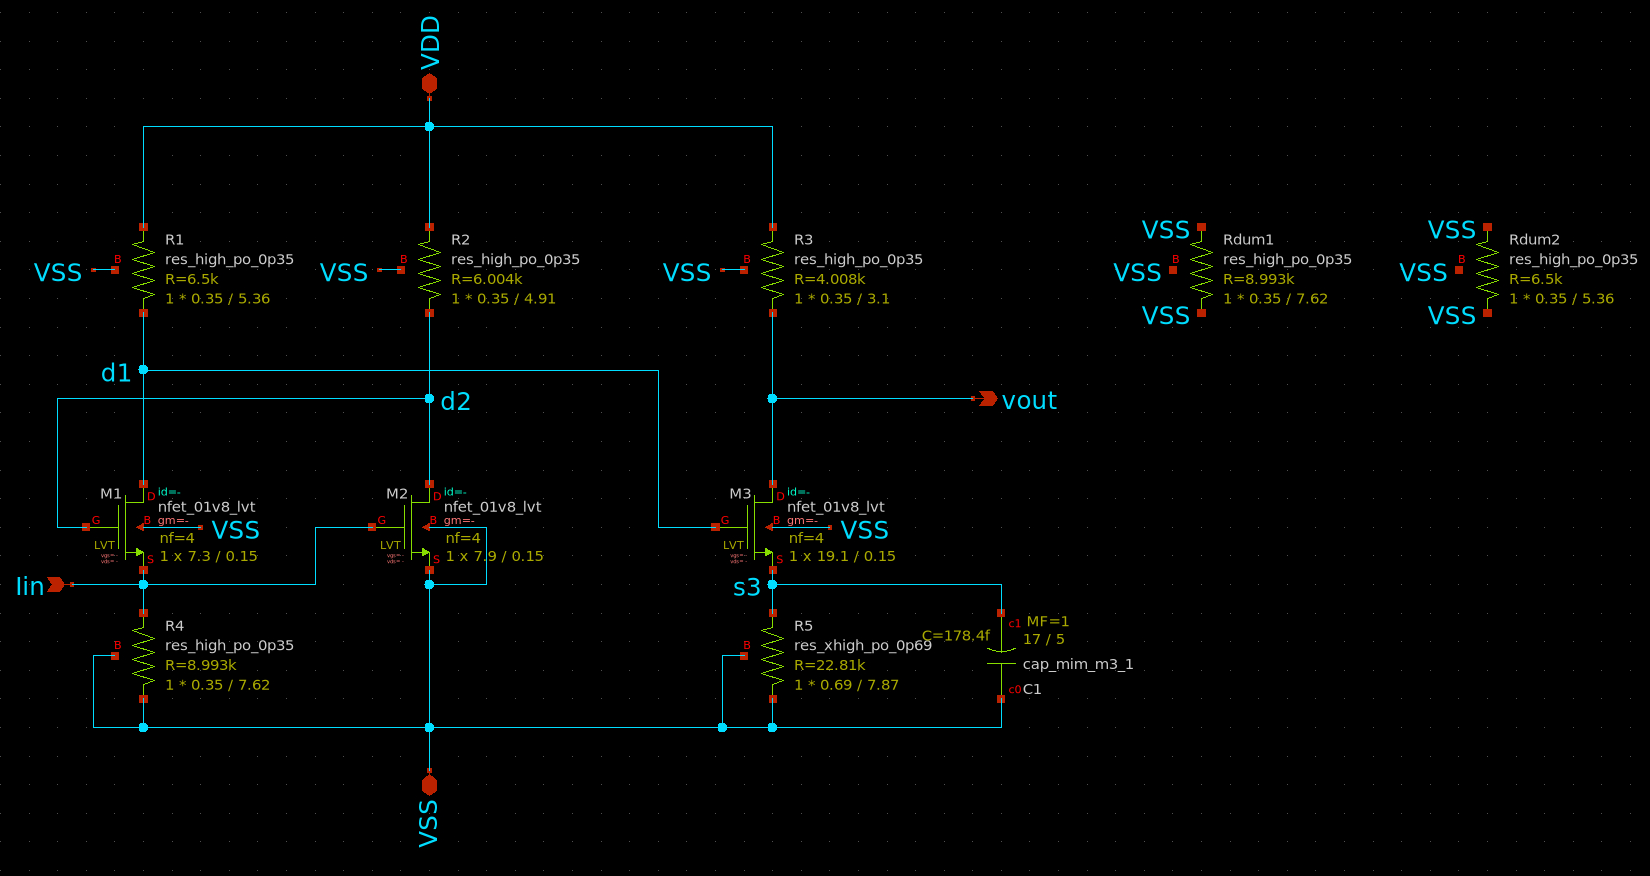
\includegraphics[width=15cm]{Figures/TIA_Xschem_Schematic.png}
\caption{RGC-CD TIA captured in \texttt{xschem}: signal devices $M_1$--$M_3$
(\texttt{nfet\_01v8\_lvt}, $n_f=4/4/4$), the $R_1$--$R_5$ poly-resistor bias network with two
flanking dummies, and the MIM degeneration capacitor $C_1$. This schematic drives both the
pre-layout simulation and the LVS comparison.}
\label{fig:xschem}
\end{figure}

\subsection{Layout (\texttt{magic})}
\label{sec:layout}
The cell was laid out in \texttt{magic} on the SKY130A PDK (Figure~\ref{fig:magic}). The three
signal transistors are folded ($n_f=4/4/4$, Section~\ref{sec:fingering}) with interdigitated
fingers sharing source/drain diffusions. The poly resistors form a matched bank, the MIM
degeneration capacitor sits alongside, and a substrate guard ring encloses the whole cell to
fix the well/substrate potential. The completed core measures
$25.46\,\mu\text{m}\times9.8\,\mu\text{m}$ ($\approx250\,\mu\text{m}^2$), compact enough to be
replicated per MVM column, which was the original area motivation for the RGC front-end
(Section~\ref{sec:prior}).

\begin{figure}[H]
\centering
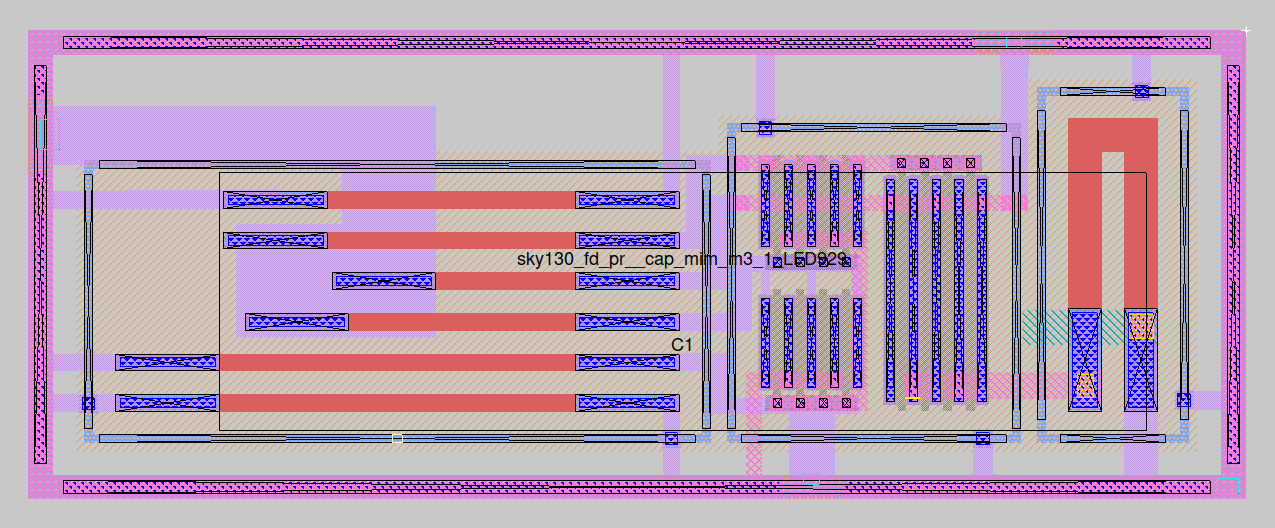
\includegraphics[width=15cm]{Figures/TIA_Magic_Layout.png}
\caption{Finished \texttt{magic} layout of the RGC-CD TIA ($25.46\times9.8\,\mu$m): the folded
$M_1$--$M_3$ transistor array, the matched poly-resistor bias bank, and the MIM degeneration
capacitor, all enclosed by a substrate guard ring.}
\label{fig:magic}
\end{figure}

\subsection{Dummy Resistors and Bank Matching}
\label{sec:dummies}
The bias resistors $R_1$--$R_4$ set the operating point and the pole/zero locations, so their
\emph{ratios} matter more than their absolute values. To keep those ratios accurate the four
active resistors are drawn as a single matched bank of parallel \texttt{res\_high\_po\_0p35}
strips on a common orientation and pitch. The dominant systematic error such a bank has to reject
is the \emph{edge effect}: the outermost strip in an array etches and planarises differently from
an interior strip, because it sees open field on one side instead of an identical neighbour. Left
uncorrected this skews the two edge resistors and breaks the very ratios the bank exists to hold.

The two dummy resistors \texttt{Rdum1} and \texttt{Rdum2} exist solely to absorb that edge error.
They flank the bank on either side (bank order, bottom to top:
\texttt{Rdum1}, $R_4$, $R_2$, $R_3$, $R_1$, \texttt{Rdum2}) so that every \emph{active} resistor is
bracketed by identical poly neighbours on both sides and no signal-setting device sits on the
array edge. The dummies carry no signal (both terminals of each are tied to \texttt{VSS}), so
they are electrically inert and appear in the netlist only as grounded devices. Their entire
purpose is geometric, to reproduce the local environment (spacing, poly density, well proximity)
that the interior strips enjoy.

For the matching to work each dummy need only replicate the environment its \emph{nearest active
neighbour} sees, which means matching that neighbour's length rather than being made arbitrarily
tall. This is also a manufacturability requirement, not just a nicety. In SKY130 the resistor
mask (\texttt{rpm}, GDS 86/20) is \emph{generated} from the poly-resistor bodies at GDS write and
merges across adjacent strips of similar height. A dummy left taller than its short neighbour
leaves an isolated \texttt{rpm} finger narrower than the $1.27\,\mu$m minimum, which fails the
\texttt{rpm.1a} width rule. Length-matching each dummy to its neighbour, \texttt{Rdum1} to
$R_4$ ($L=7.62\,\mu$m) and \texttt{Rdum2} to $R_1$ ($L=5.36\,\mu$m), removes that protruding
finger and closes the DRC at its source, while still presenting each edge resistor with a
full-length matched neighbour. The result is clean sign-off DRC with the bank's matching
integrity intact.

\subsection{Layout-vs-Schematic (LVS)}
\label{sec:lvs}
LVS was run with \texttt{netgen}, comparing the \texttt{magic}-extracted device netlist against
the \texttt{xschem} schematic netlist. The comparison caught two real layout errors before it
closed: the input node $Iin$ inadvertently shorted to \texttt{VSS}, and a signal transistor
drawn at $4\times$ its intended width. Both were fixed in the layout. The final run
reports \emph{netlists match uniquely}: 10 devices and 7 nets on each side, equivalent cell pin
lists (\texttt{Iin}, \texttt{Vout}, \texttt{VDD}, \texttt{VSS}), and no property mismatches. The
layout is therefore a verified electrical match to the design of record.

\subsection{Parasitic Extraction and Post-Layout Simulation}
\label{sec:pex}
With LVS clean, \texttt{magic} extracted a post-layout netlist including parasitic capacitance.
This first pass is \emph{cap-only}: it captures coupling and substrate capacitance on every net
(105 parasitic $C$ elements) but not wire or gate resistance, which is the standard first pass
and models the dominant post-layout effect: the extra node capacitance loading the
high-impedance internal nodes. The post-layout testbenches re-inject the same
$C_T=500\,fF$/$C_L=1\,pF$ loading used pre-layout.

As expected, the parasitics leave the bias untouched: the post-layout operating point settles at
$V_{in}=0.63\,V$, $V_{out}=1.67\,V$, and $I_{tot}=0.171\,mA$ ($0.31\,mW$), tracking the
pre-layout sim. The loaded frequency response (the dash-dot trace of
Figure~\ref{fig:freq response}) holds its DC transimpedance at $59.6\,dB\Omega$ while the added
node capacitance trims the $-3\,dB$ bandwidth from the folded-device $603\,MHz$ to $556\,MHz$
(a further ${\sim}8\%$, for a cumulative $-12\%$ from the ideal $631\,MHz$) and lifts peaking to
a still-benign $0.22\,dB$. Table~\ref{tab:pex} collects the progression. The design is robust to
its own layout parasitics: the capacitive-degeneration compensation survives extraction with the
flat, well-damped response intact.

\begin{table}[H]
    \centering
    \caption{Loaded response through the physical-implementation flow (SKY130A, TT, $27^\circ$C,
    $C_T=500\,fF$, $C_L=1\,pF$).}
    \label{tab:pex}
    \begin{tabular}{l|c|c|c} \hline
        \textbf{Metric} & \textbf{Ideal ($n_f{=}1$)} & \textbf{Real devices (folded)} & \textbf{Post-layout (PEX)} \\ \hline
        DC transimpedance [$dB\Omega$] & 59.4 & 59.6 & 59.6 \\ \hline
        Loaded $f_{-3dB}$ [MHz]        & 631  & 603  & 556  \\ \hline
        Peaking [dB]                   & $<0.1$ & $<0.1$ & 0.22 \\ \hline
        Supply current [mA]            & 0.18 & 0.18 & 0.171 \\ \hline
    \end{tabular}
\end{table}

Two extraction caveats remain. The pass is cap-only: wire and gate resistance (and hence the
fingering noise benefit of Section~\ref{sec:fingering}) are not modelled directly, as
\texttt{magic}'s \texttt{extresist} does not converge on the high-resistance poly nets of this
cell. Their bandwidth impact is nonetheless bounded to be negligible: inserting a series
resistance at the output node (which drives the dominant $1\,pF$ load, making it the most
resistance-sensitive node in the circuit) shows that even a pessimistic $50\,\Omega$ of
interconnect (well above the few-to-tens of ohms expected on this compact layout) trims the
bandwidth by under $1.5\%$ ($556\to548\,MHz$) at unchanged DC gain, and if anything slightly
\emph{reduces} peaking by damping the loop. The second caveat: loop phase margin cannot be
measured directly on the raw extracted netlist, because the $M_1$--$M_2$ regulation node that the
pre-layout testbench breaks for injection is a single physical net in the layout. Checking it
requires splitting that node in the extracted deck.

\section{Conclusion and Future Work}
This report documented the hand design, small-signal analysis, open-source simulation, and
physical implementation (schematic capture, layout, LVS, and parasitic extraction) of a
regulated-cascode TIA with a capacitive-degeneration bandwidth-extension stage. The original
SKY130B baseline (Section~\ref{sec:prior}) was revitalised on SKY130A by discarding the
overdrive-voltage sizing in favour of a $g_m/I_D$ methodology (Section~\ref{sec:flow}). The
result is a $59.4\,dB\Omega$ transimpedance that, once the CD zero is placed on the ADC-load
pole, holds flat out to $631\,MHz$ at only $0.33\,mW$ (a $3\times$ power reduction over the
baseline) with $\approx130^\circ$ of loop phase margin. The design was then laid out in
\texttt{magic}, closed LVS, and re-simulated with parasitic extraction (Section~\ref{sec:physical}),
where the post-layout bandwidth settles at $556\,MHz$ at unchanged gain. The chief remaining limitations are
the asymmetric single-ended output swing (Section~\ref{sec:linearity}) and the sensitivity of
the CD compensation to the actual load.

As a visual capstone of that back-end flow, Figure~\ref{fig:gds render} renders the signed-off
GDS of Section~\ref{sec:layout} as a full process stack: (a) an \emph{exploded} view that
separates the layers vertically (the nwell/diffusion base, the poly and local-interconnect
level, and the five metal layers with their connecting vias) and (b) the same stack collapsed
into its as-fabricated form. The tight, near-square footprint that motivated the RGC front-end
in the first place (Sections~\ref{sec:prior} and~\ref{sec:layout}) is apparent in how few metal
levels the routing actually consumes.

\begin{figure}[H]
\centering
\begin{minipage}[b]{0.48\textwidth}
\centering
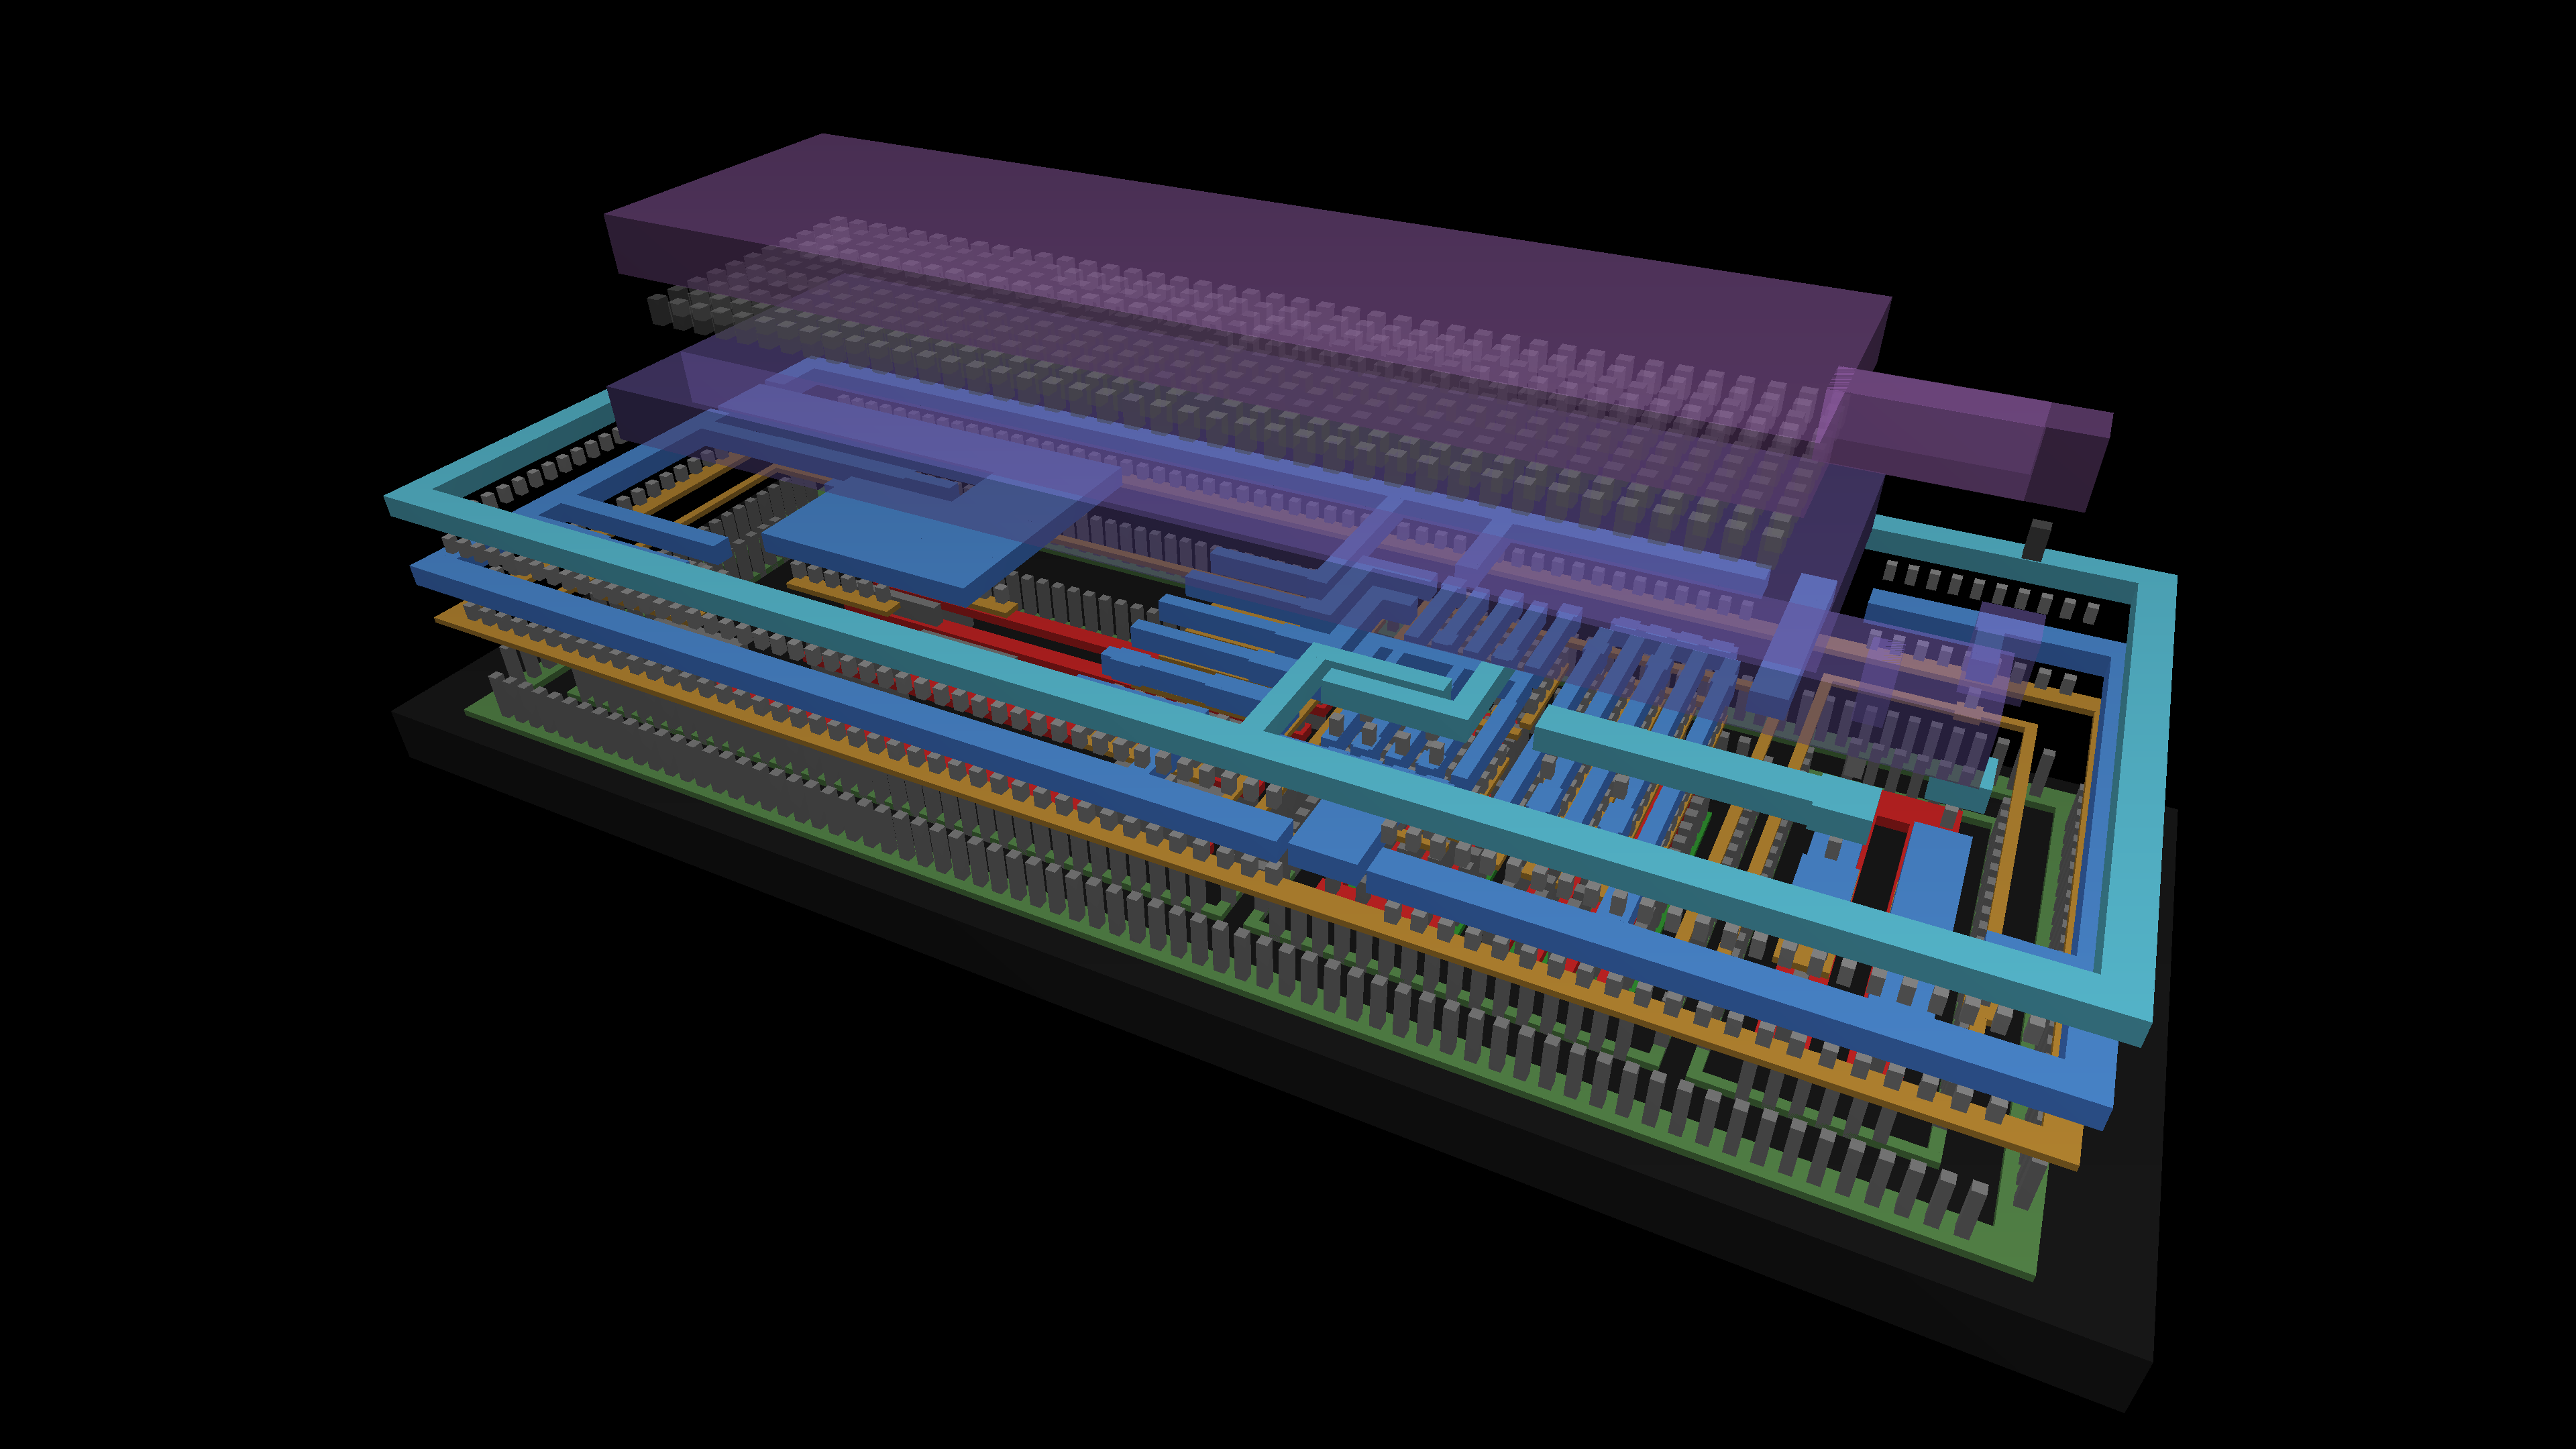
\includegraphics[width=\textwidth]{Figures/TIA-GDS-Exploded.png}
\\{\footnotesize (a) exploded layer stack}
\end{minipage}
\hfill
\begin{minipage}[b]{0.48\textwidth}
\centering
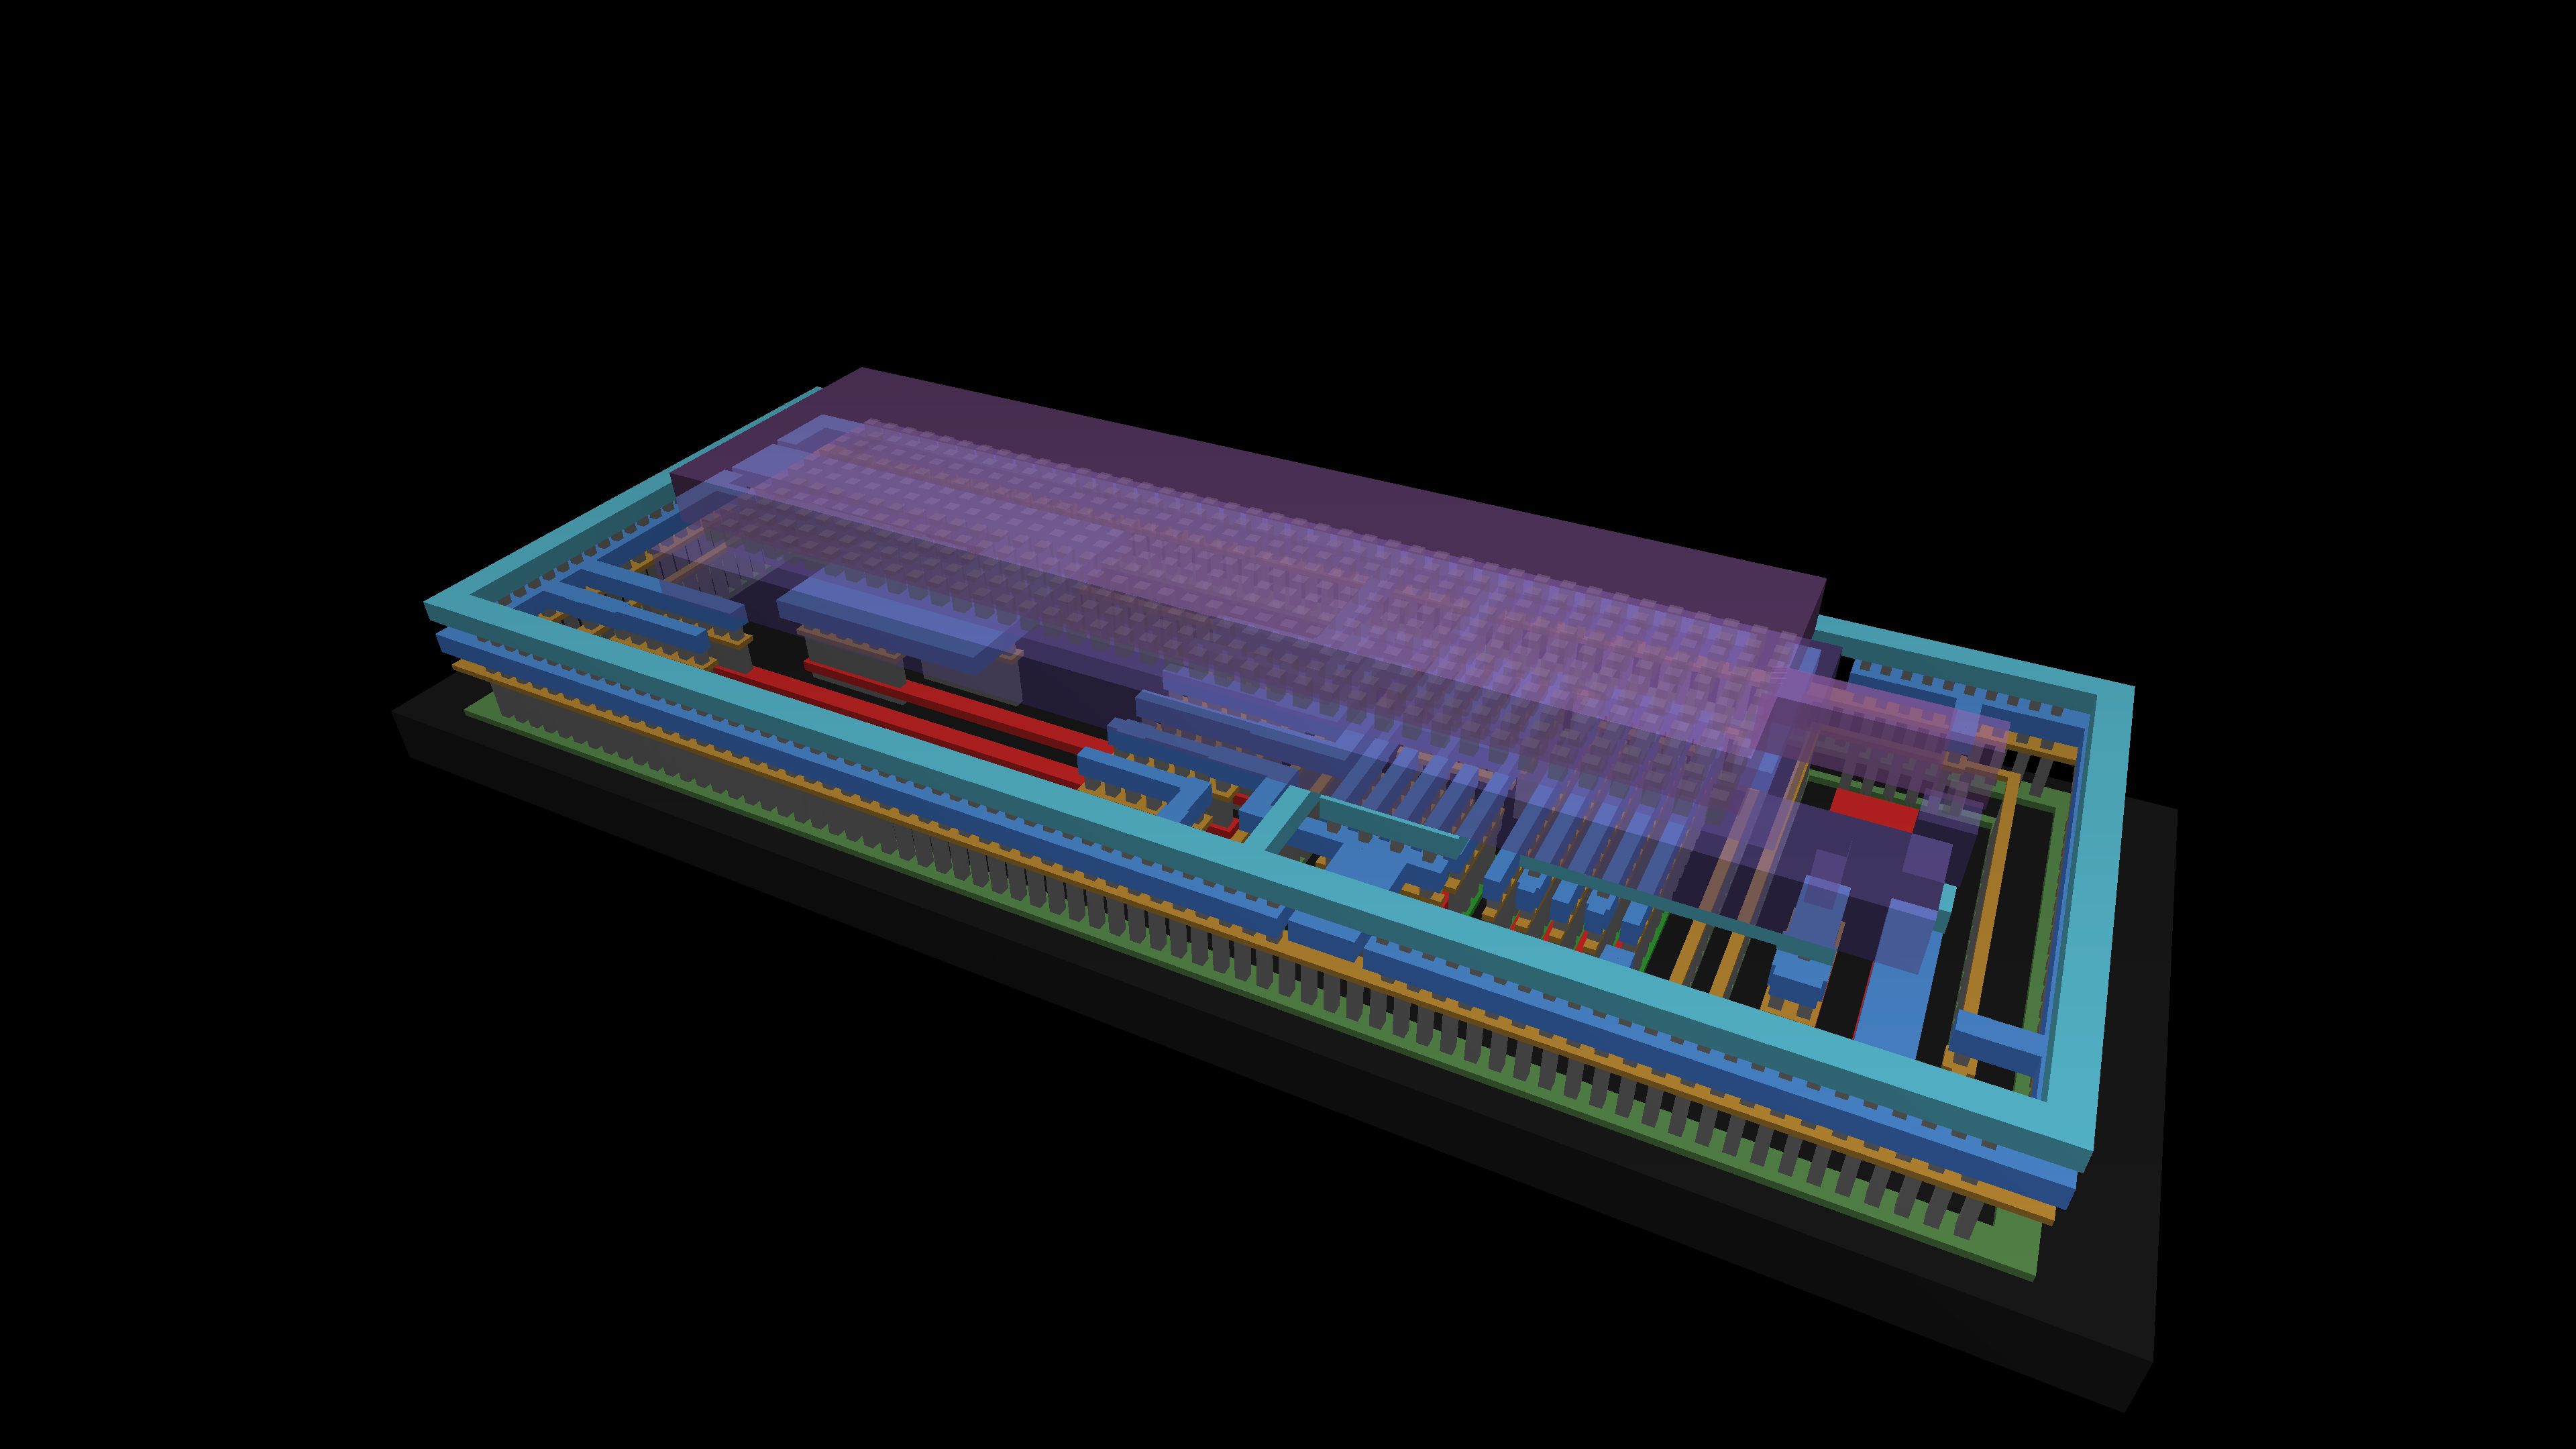
\includegraphics[width=\textwidth]{Figures/TIA-GDS-3D.png}
\\{\footnotesize (b) as-fabricated stack}
\end{minipage}
\caption{Three-dimensional render of the signed-off RGC-CD TIA GDS: (a) exploded view separating
the process layers (diffusion/nwell base through poly, local interconnect, and metal1--metal5),
and (b) the collapsed as-fabricated metal stack. Both are the same $25.46\times9.8\,\mu$m cell of
Figure~\ref{fig:magic}.}
\label{fig:gds render}
\end{figure}

Future work:
\begin{itemize}
    \item \textbf{Symmetric operation:} bias the output at $\approx V_{DD}/2$ for balanced swing,
    or adopt a (pseudo-)differential TIA to support true signed bidirectional input currents.
    \item \textbf{Load co-design:} fix the CD zero against the real, extracted current-mirror
    input and ADC load capacitances so the reported bandwidth reflects the true dominant pole.
    \item \textbf{Process comparison:} port the $g_m/I_D$ design back to SKY130B and A/B the two
    model sets to quantify the transconductance and parasitic differences.
    \item \textbf{Full extraction:} extend the cap-only PEX of Section~\ref{sec:pex} to a full RC
    extraction (adding wire and gate resistance, and with it the fingering noise benefit), and
    re-check the regulation-loop phase margin on the extracted netlist.
\end{itemize}

\appendix
\section{Appendix: Input-Architecture Comparison Study}
\label{app:arch}
This study pre-dates the finalised design. It was an early exploration at a higher
$\sim$1.15 mW operating point with \emph{unloaded} testbenches (no $C_T/C_L$) and noise
integrated over the old $144\,MHz$ band, so its absolute numbers do not match the
$g_m/I_D$ design of record of Section~\ref{sec:flow} ($0.33\,mW$, $59.4\,dB\Omega$, loaded
to $631\,MHz$). In particular its ``Baseline'' is the original RGC at that operating point,
not the finalised converter. What carries over is the \emph{relative} comparison between
topologies and the qualitative findings below, not the tabulated absolutes.

To evaluate the biasing, gain-definition and noise trade-offs raised in the
conclusion, four TIA input architectures were prototyped in ngspice on SKY130A.
All share a $1.8\ V$ supply and a $\sim$1.15 mW budget, and use identical
testbenches: transimpedance and input impedance are read from a $1\ A$ AC probe
at the input ($|V_{out}|=|Z_T|$, $|V_{in}|=|Z_{in}|$), and input-referred current
noise is integrated over $1\ kHz$--$144\ MHz$. The variants are:
\begin{itemize}
    \item \textbf{Baseline:} the original RGC with resistor-divider biasing.
    \item \textbf{A: Shunt-feedback:} the RGC is \emph{removed} and replaced by
    a single inverting common-source stage (NMOS input, PMOS current-source load)
    with a feedback resistor $R_f$ from output to input, giving $Z_T\approx -R_f$ and
    $Z_{in}\approx R_f/(1+A)$.
    \item \textbf{B: Hybrid:} the baseline RGC with an additional \emph{global},
    AC-coupled feedback resistor from output back to the input node (nested loops).
    \item \textbf{C: Current-mirror-biased RGC:} the baseline signal path with
    the input-tail current set by an ideal reference (a proxy for a matched current
    mirror from a bandgap) in place of $R_4$.
\end{itemize}

\begin{table}[H]
    \centering
    \caption{Architecture comparison (SKY130A, TT, $27^oC$, $\sim$1.15 mW each)}
    \label{tab:arch}
    \begin{tabular}{l|c|c|c|c} \hline
        \textbf{Metric} & \textbf{Baseline} & \textbf{A: Shunt-fb} & \textbf{B: Hybrid} & \textbf{C: CM-bias} \\ \hline
        $Z_T$ [$dB\Omega$] ($\Omega$) & 63.5 (1502) & 61.4 (1178) & 49.5 (298) & 63.7 (1537) \\ \hline
        $Z_{in}$ [$\Omega$] & 47 & 322 & 39 & 48 \\ \hline
        Peaking [dB] & 0.54 & \textbf{0.02} & 2.73 & 0.69 \\ \hline
        $f_{-3dB}$ & 6.9 GHz & 5.0 GHz & 20 GHz & 7.3 GHz \\ \hline
        $I_{noise}$ [$nA_{rms}$] & 115 & \textbf{60} & 234 & 107 \\ \hline
        Power [mW] & 1.15 & 1.16 & 1.15 & 1.15 \\ \hline
    \end{tabular}
\end{table}

Note that the absolute $f_{-3dB}$ values are unrealistically high because these
pre-layout testbenches include no input or load capacitance (Section
\ref{sec:tf}). The \emph{comparison} between architectures is the
meaningful result, not the absolute bandwidth.

\subsection{PVT Observations}
Across the ss/tt/ff corners the transimpedance of every RGC-based variant moves by
only $\sim$0.5 dB, because $Z_T\approx R_1$ is set by a resistor rather than by
device transconductance. The original design's \emph{gain} is therefore more
PVT-robust than expected. The unregulated quantity is the \emph{bias current}: a
$\pm10\%$ supply sweep (Table \ref{tab:vdd}) moves the total current by $+44\%$,
since with resistor loads $I_D\propto V_{DD}$.

\begin{table}[H]
    \centering
    \caption{Total supply current vs.\ supply voltage ($\pm10\%$, TT)}
    \label{tab:vdd}
    \begin{tabular}{l|c|c|c|c} \hline
        \textbf{Architecture} & \textbf{1.62 V} & \textbf{1.80 V} & \textbf{1.98 V} & \textbf{Spread} \\ \hline
        Baseline (resistor bias)   & 0.52 mA & 0.64 mA & 0.75 mA & $+44\%$ \\ \hline
        C (tail current mirror)    & 0.53 mA & 0.64 mA & 0.75 mA & $+42\%$ \\ \hline
    \end{tabular}
\end{table}

Crucially, current-mirror biasing the input tail alone (variant C) barely improves
this: the load resistors $R_1$--$R_3$ still set the M2/M3 branch currents, which
continue to scale with $V_{DD}$. In this resistor-loaded topology the load devices
do double duty as bias-setting elements, so the bias cannot be robustified without
replacing them with current-source loads plus common-mode feedback, which
amounts to a different architecture.

\subsection{Findings}
\begin{itemize}
    \item \textbf{A (shunt-feedback) is the strongest architecture:} the flattest
    response ($0.02\ dB$ peaking), roughly half the input-referred noise
    ($60$ vs $115\ nA_{rms}$), and a transimpedance defined by a single resistor
    $R_f$. Its only weakness is a higher input impedance ($322\ \Omega$), caused by
    the modest loop gain of a single-stage forward amplifier
    ($Z_{in}=R_f/(1+A)$, $A\approx4$). \textbf{Cascoding the forward stage} raises
    $A$ and restores a low $Z_{in}$. Importantly, this forward amplifier is a small
    (one- to few-transistor) inverting stage, \emph{not} a full operational
    amplifier, so it preserves the area advantage that motivated the RGC choice.
    \item \textbf{B (hybrid) is counterproductive:} the global loop collapses the
    transimpedance to $49.5\ dB\Omega$, doubles the noise ($234\ nA_{rms}$), and
    raises peaking to $2.7\ dB$. Nested local + global feedback is not worthwhile
    here. This penalty is fundamental rather than a testbench artefact: the global
    $R_f$ forms a second shunt path that competes with the existing local RGC
    regulation, simultaneously subtracting from the forward transimpedance and
    injecting its own thermal noise at the summing node, so the result holds
    independent of the load ($C_T$, $C_L$) and does not warrant re-evaluation on the
    loaded RGC-CD.
    \item \textbf{C (CM-biased RGC) $\approx$ baseline:} essentially unchanged
    signal performance and, as shown above, little bias-robustness gain, a
    consequence of the resistor-load coupling rather than a flaw in the idea.
\end{itemize}

\bibliographystyle{IEEEtran}
\bibliography{Sources}

\end{document}
